\documentclass{beamer}


%->8-------------------------------------------------------------------------------------------8<-%
\usepackage[brazil]{babel}
\usepackage[utf8]{inputenc}
\usepackage[T1]{fontenc}
%->8-------------------------------------------------------------------------------------------8<-%

%->8-------------------------------------------------------------------------------------------8<-%
\usetheme{Darmstadt}
%->8-------------------------------------------------------------------------------------------8<-%

%->8-------------------------------------------------------------------------------------------8<-%
\usepackage{graphicx}
\usepackage{float}
%->8-------------------------------------------------------------------------------------------8<-%

%->8-------------------------------------------------------------------------------------------8<-%
\usepackage{geometry}
\geometry{left=0.4cm, right=0.4cm}
\usepackage{csquotes}
\usepackage{upquote}
\usepackage{listings}
\usepackage{hyperref}
\setbeamertemplate{navigation symbols}{}
\setbeamertemplate{footline}{\quad\hfill\normalsize{\insertframenumber}\strut\quad\,}
%->8-------------------------------------------------------------------------------------------8<-%

%->8-------------------------------------------------------------------------------------------8<-%
\usepackage[style=numeric, backend=biber]{biblatex}
\addbibresource{outer-crust/repertoire.bib}
\graphicspath{{figures}}
%->8-------------------------------------------------------------------------------------------8<-%

%->8-------------------------------------------------------------------------------------------8<-%
\lstnewenvironment{code}[1][]{
  \lstset{
    basicstyle=\ttfamily,
    columns=flexible,
    breaklines=true,
    breakatwhitespace=true,
    frame=none,
    basewidth=0.5em,
    aboveskip=13pt,
    belowskip=0pt,
    #1
  }
}{}

\newcommand{\excerptpage}[2]{
  \begin{center}
    \textit{#1}\\
        --- #2.
  \end{center}
}

\newcommand{\bigtitlepage}[1]{%
  \section{#1}
  \begin{center}
    \vspace*{\fill}
    {\Huge #1}
    \vspace*{\fill}
  \end{center}
}
%->8-------------------------------------------------------------------------------------------8<-%

% Math
%->8-------------------------------------------------------------------------------------------8<-%
\usepackage{amsmath, amssymb, calculation, mathdots, scalerel, mathtools}
\usepackage{../calculation}

  % Matrices and Vectors Related Commands
  %->8-------------------------------------------------------------8<-%
  \newenvironment{jmatrix}{\left[\begin{matrix}}{\end{matrix}\right]}
  \newcommand{\norm}[1]{\left\lVert#1\right\rVert}
  \newcommand{\fnorm}[1]{\left\lVert#1\right\rVert_\mathsf{F}}
  \newcommand{\dotprod}[2]{\left\langle #1 \, \middle| \, #2 \right\rangle}
  \newcommand{\proj}[2]{\mathrm{proj}_{#1}(#2)}
  \renewcommand{\det}[1]{\mathrm{det}\left(#1\right)}
  \newcommand{\posto}[1]{\mathrm{posto}\left(#1\right)}
  \newcommand{\dist}[1]{\mathrm{dist}(#1)}
  \newcommand{\N}[1]{\mathrm{N}\left(#1\right)}
  \newcommand{\spn}[1]{\mathrm{span}\left(#1\right)}
  \renewcommand{\t}{^{\scriptscriptstyle\mathsf{T}\mkern-1mu}}
  \renewcommand{\dim}[2]{(#1 \times #2)}
  \newcommand{\bigvert}{\rule[-1ex]{0.5pt}{6.8ex}}
  \renewcommand{\vert}{\rule[-1ex]{0.5pt}{2.5ex}}
  \newcommand{\bighori}{\rule[.5ex]{6.8ex}{0.5pt}}
  \newcommand{\hori}{\rule[.5ex]{2.5ex}{0.5pt}}
  %->8-------------------------------------------------------------8<-%

  % Optimization Related Commands
  %->8-------------------------------------------------------------8<-%
  \newcommand{\mintext}{\text{Min}}
  \renewcommand{\min}[1]{\underset{#1}{\mathrm{Min}}\,\,}
  \newcommand{\maxtext}{\text{Max}}
  \renewcommand{\max}[1]{\underset{#1}{\mathrm{Max}}\,\,}
  \newcommand{\argmintext}{\text{Argmin}}
  \newcommand{\argmin}[1]{\underset{#1}{\mathrm{Argmin}}\,\,}
  \newcommand{\argmaxtext}{\text{Argmax}}
  \newcommand{\argmax}[1]{\underset{#1}{\mathrm{Argmax}}\,\,}
  %->8-------------------------------------------------------------8<-%

  % Functions Related Commands
  %->8-------------------------------------------------------------8<-%
  \newcommand{\grad}[1]{\underset{#1}{\nabla}\,\,}
  \newcommand{\hess}[1]{\underset{#1}{\mathcal{H}}\,\,}
  \newcommand{\sderiv}[2]{\dfrac{d #2}{d #1}}
  \newcommand{\bderiv}[2]{\dfrac{d}{d #1}\left(#2\right)}
  \newcommand{\spderiv}[2]{\dfrac{\partial #2}{\partial #1}}
  \newcommand{\bpderiv}[2]{\dfrac{\partial}{\partial #1}\left(\displaystyle#2\right)}
  \newcommand{\dpderiv}[2]{\dfrac{\partial^2\left(\displaystyle#2\right)}{\partial #1^2}}
  \newcommand{\vero}[1]{\mathcal{L}(#1)}
  \newcommand{\cvero}[2]{\mathcal{L}(#1 \mid #2)}
  \newcommand{\prob}[2]{\mathrm{P}_{#1}\left[#2\right]}
  \newcommand{\cprob}[3]{\mathrm{P}_{#1}\left(#2 \mid #3\right)}
  \newcommand{\pfunc}[2]{\mathrm{P}_{#1}\left(#2\right)}
  %->8-------------------------------------------------------------8<-%

  % Number Related Commands
  %->8-------------------------------------------------------------8<-%
  \newcommand{\mul}{\cdot}
  \renewcommand{\deg}{\ensuremath{^\circ}}
  \renewcommand{\sin}[1]{\mathrm{sen}\left(#1\right)}
  \newcommand{\logtext}{\mathrm{log}}
  \renewcommand{\log}[1]{\logtext\left(#1\right)}
  \newcommand{\lntext}{\mathrm{ln}}
  \renewcommand{\ln}[1]{\lntext\left(#1\right)}
  \renewcommand{\exp}[1]{\mathrm{e}^{#1}}
  \newcommand{\abs}[1]{\left\lvert#1\right\rvert}
  %->8-------------------------------------------------------------8<-%

  % Modeling Related Commands
  %->8-------------------------------------------------------------8<-%
  \newcommand{\blackbox}{\raisebox{0.2ex}{\rule{1.2ex}{1.2ex}}}
  \newcommand{\whitebox}{\raisebox{0.2ex}{\fboxsep=0pt\fbox{\rule{1.2ex}{0pt}\rule{0pt}{1.2ex}}}}
  \newcommand{\fim}[2]{\vspace{0.075cm} \dfrac{#1}{#2}}
  %->8-------------------------------------------------------------8<-%

  % Other Math Related Commands
  %->8-------------------------------------------------------------8<-%
  \newcommand{\rep}[1]{\mathrm{rep}\left(#1\right)}
  % \newcommand{\union}{\cup}
  \newcommand{\bigunion}{\bigcup}
  % \newcommand{\intersec}{\cap}
  \newcommand{\bigintersec}{\bigcap}
  % \renewcommand{\gets}{\leftarrow}
  \newcommand{\E}{\Sigma}
  \newcommand{\st}{\,\,|\,\,}
  \newcommand{\bigst}{\,\,\,\,\rule[-0.5cm]{0.5pt}{6.8ex}\,\,\,\,}
  \newcommand{\impliesdown}{\displaystyle\Downarrow}
  % \DeclareMathOperator*{\com}{\scalerel*{,}{\sum}}
  %->8-------------------------------------------------------------8<-%
%->8-------------------------------------------------------------------------------------------8<-%

%->8-------------------------------------------------------------------------------------------8<-%
\title{Raciocínio Equacional para a Derivação de \\ Algoritmos de Álgebra Linear sob a \\ Perspectiva de Otimização}
\author{%
  \textbf{João Victor Lopez Pereira} \\
  \vspace{0.2cm}
  Daniel Sadoc Menasche \\
  \vspace{0.2cm}
  João Antonio Recio Paixão
}
\institute{Instituto de Computação -- UFRJ}
\date{Outubro de 2026}
%->8-------------------------------------------------------------------------------------------8<-%


\begin{document}

  \frame{\titlepage}

  \section{Mínimos Quadrados}
    
\begin{frame}{O que é Mínimos Quadrados?}

  \[
    \underbrace{\begin{aligned}
      5 x + 3 y &\approx 10, \\
      2 x + 4 y &\approx 8, \\
      3 x + 5 y &\approx 12.
    \end{aligned}}_{Ax \approx b}
  \]

  \vspace{0.1cm} \pause

  \[
    (\bar{x},\bar{y}) \in \argmin{x, y} (5 x + 3 y - 10)^2 + (2 x + 4 y - 8)^2 + (3 x + 5 y - 12)^2
  \]

  \vspace{-0.3cm}\pause

  \begin{figure}
    \centering
    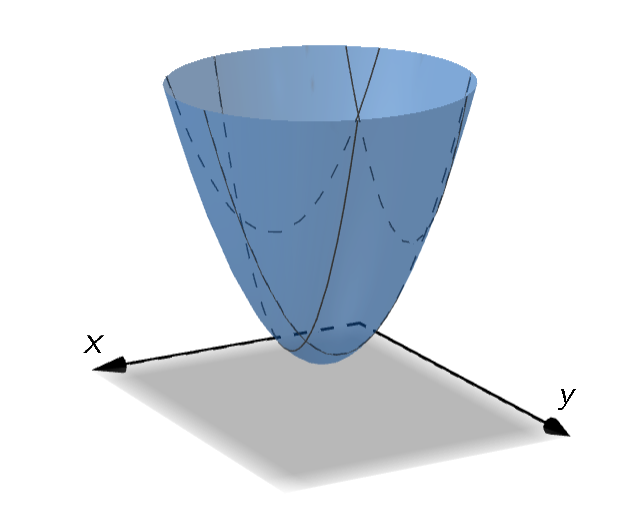
\includegraphics[width=0.4\textwidth]{paraboloid.png}
  \end{figure}

\end{frame}
    
\begin{frame}[fragile]{Mínimos Quadrados com 1 Variável}

  \[
    \begin{aligned}
      2 x &\approx 2, \\
      1 x &\approx 1, \\
      1 x &\approx 4.
    \end{aligned}
  \]

  \vspace{0.25cm} \pause

  \[
    x^{*} \in \argmin{x} (2 x - 2)^2 + (1 x - 1)^2 + (1 x - 4)^2
  \]

  \pause

  \begin{figure}
    \centering
    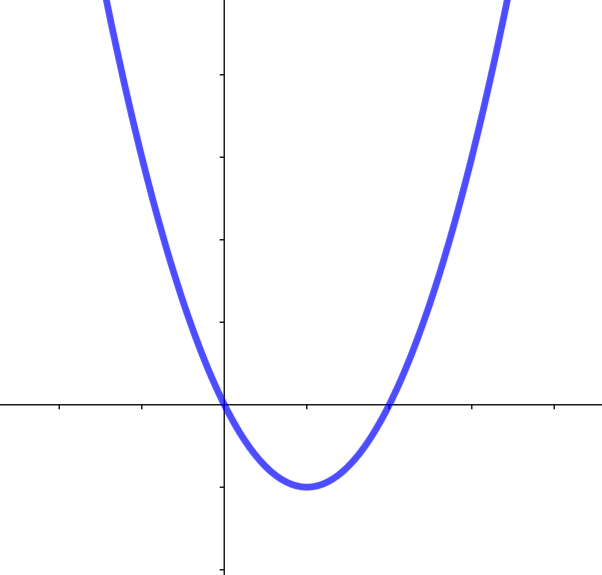
\includegraphics[width=0.3\textwidth]{parabola.png}
  \end{figure}

\end{frame}
    
\begin{frame}{Como fazer Mínimos Quadrados com Várias Variáveis?}

  \begin{itemize}
    \item Cálculo 2 (usando gradientes), \\[0.5cm]
    \item Projeções ortogonais, \\[0.5cm]
    \item Propriedades de produto interno.
  \end{itemize}

  \vspace{1cm} \pause

  \begin{itemize}
    \item Muitos pré-requisitos, \\[0.5cm]
    \item É difícil trabalhar com essas ferramentas. \\[0.5cm]
  \end{itemize}

\end{frame}

  \section{Ferramenta}
    
\begin{frame}{Propriedade de Argmin}

  \begin{lemma}[Argmin Desacoplado]
    Seja $f : X \times Y \mapsto \mathbb{R}$ uma função tal que, $\forall x \in X$, $\min{y} f(x,y)$ exista.
    \[
      \argmin{x \in X, y \in Y} f(x,y)
      =
      \left\{(\bar{x}, \bar{y}) \bigst
        \begin{array}{ll}
          \bar{x} \in \argmin{x} \min{y} f(x,y), \\
          \bar{y} \in \argmin{y} f(\bar{x}, y).
        \end{array}
      \right\}.
    \]
  \end{lemma}

\end{frame}

  \section{Solução de Mínimos Quadrados}
    
\begin{frame}[fragile]{Resolvendo Mínimos Quadrados}
  \begin{theorem}[Solução de Mínimos Quadrados]
    Seja $A \in \mathbb{R}^{m \times n}$ uma matriz e $b \in \mathbb{R}^{m}$ um vetor. Então existem matrizes $T \in \mathbb{R}^{n \times m}$ e $M \in \mathbb{R}^{n \times m}$ tais que
    \[
      (\bar{x}, \bar{v})
      \in
      \am{x} \norm{Ax - b}
      \iff
      \bar{x} = T b \text{ e } \bar{v} = \norm{M b}.
    \]
  \end{theorem}
  \pause
  \begin{proof}
    A prova é por indução na dimensão de $x$ (número de variáveis).

    \vspace{0.6cm}

    \textbf{Caso Base:} $x=1$: Não mostraremos aqui. :)
    \renewcommand{\qedsymbol}{}
  \end{proof}
\end{frame}

\begin{frame}
  \begin{proof}
    \textbf{Passo de Indução:}
    \begin{calcproof}[]
      \start{(\bar{x_1}, \bar{x_2}, \bar{v}) \in \am{x_1, x_2} \norm{ \begin{jmatrix} A_1 & a_2 \end{jmatrix} \begin{jmatrix} x_1 \\ x_2 \end{jmatrix} - b}}
      \step{Multiplicação matriz-vetor}{
      (\bar{x_1}, \bar{x_2}, \bar{v}) \in \am{x_1, x_2} \norm{A_1 x_1 + a_2 x_2 - b}}
      \step{Argmin Desacoplado}{
      \begin{array}{ll}
        \bar{x_1} \in \argmin{x_1} \norm{A_1 x_1 + A_2 \bar{x_2} + b} \\[0.2cm]
        (\bar{x_2}, \bar{v}) \in \am{x_2} \min{x_1} \norm{A_1 x_1 + A_2 x_2 + b}
      \end{array}}
    \end{calcproof}
    \renewcommand{\qedsymbol}{}
  \end{proof}
\end{frame}

\begin{frame}
  \begin{proof}
    \begin{calcproof}[]
      \start{
      \begin{array}{ll}
        \bar{x_1} \in \argmin{x_1} \norm{A_1 x_1 + A_2 \bar{x_2} + b} \\[0.2cm]
        (\bar{x_2}, \bar{v}) \in \am{x_2} \min{x_1} \norm{A_1 x_1 + A_2 x_2 + b}
      \end{array}}
      \step{Hipótese de Indução}{
      \begin{array}{ll}
        \bar{x_1} = T_1 (- b - A_2 \bar{x_2}) \\[0.2cm]
        (\bar{x_2}, \bar{v}) \in \am{x_2} \norm{M_1 (b - A_2 x_2)}
      \end{array}}
      \step{Hipótese de Indução}{
      \begin{array}{lll}
        \bar{x_1} = T_1 (- b - A_2 \bar{x_2}) \\[0.2cm]
        \bar{x_2} = T_2 M_1 b \\[0.2cm]
        \bar{v} = \norm{M_2 M_1 b}
      \end{array}}
    \end{calcproof}
    \renewcommand{\qedsymbol}{}
  \end{proof}
\end{frame}


  \section{Outros Problemas de Otimização}
    
\begin{frame}{O Que Mais Estamos Fazendo?}

  Focamos nossa apresentação na SIAc no problema tradicional de Mínimos Quadrados, mas também estamos trabalhando em outros problemas de otimização.

  \pause

  \begin{figure}
    \begin{minipage}[t]{0.47\textwidth}
      \centering
      \vspace{-1.5cm}
      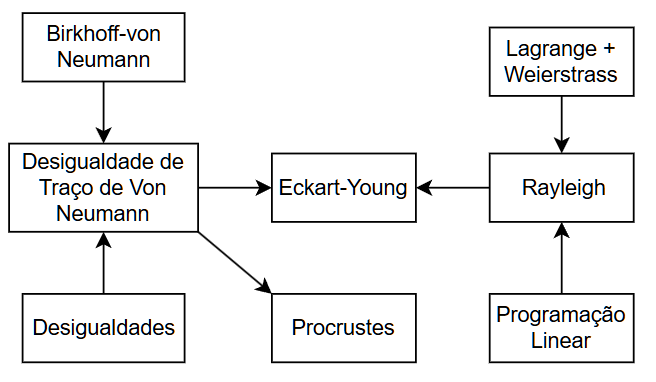
\includegraphics[width=6.5cm]{horrible-tree.png}
    \end{minipage}
    \hfill \pause
    \begin{minipage}[t]{0.47\textwidth}
      \centering
      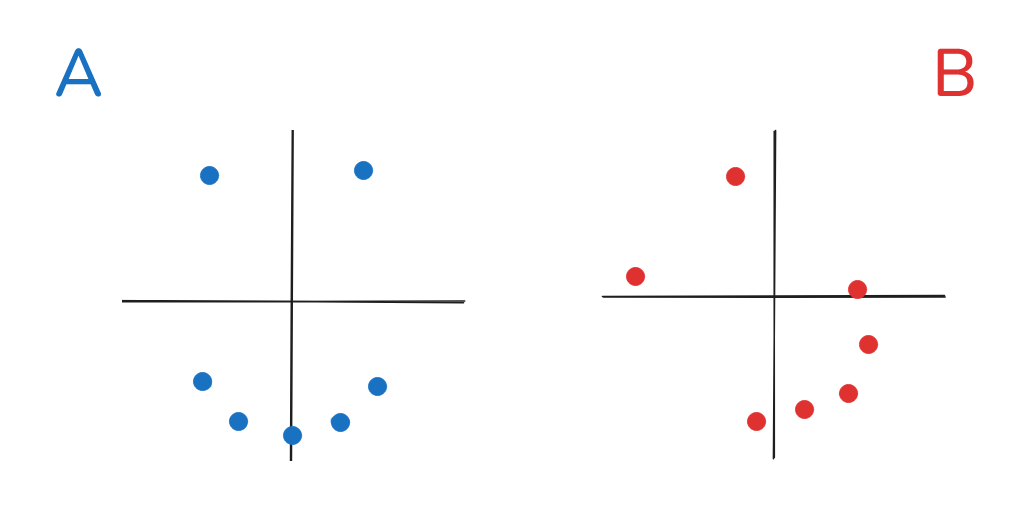
\includegraphics[width=5cm]{procrustes.png}
      \vspace{1cm} \pause
      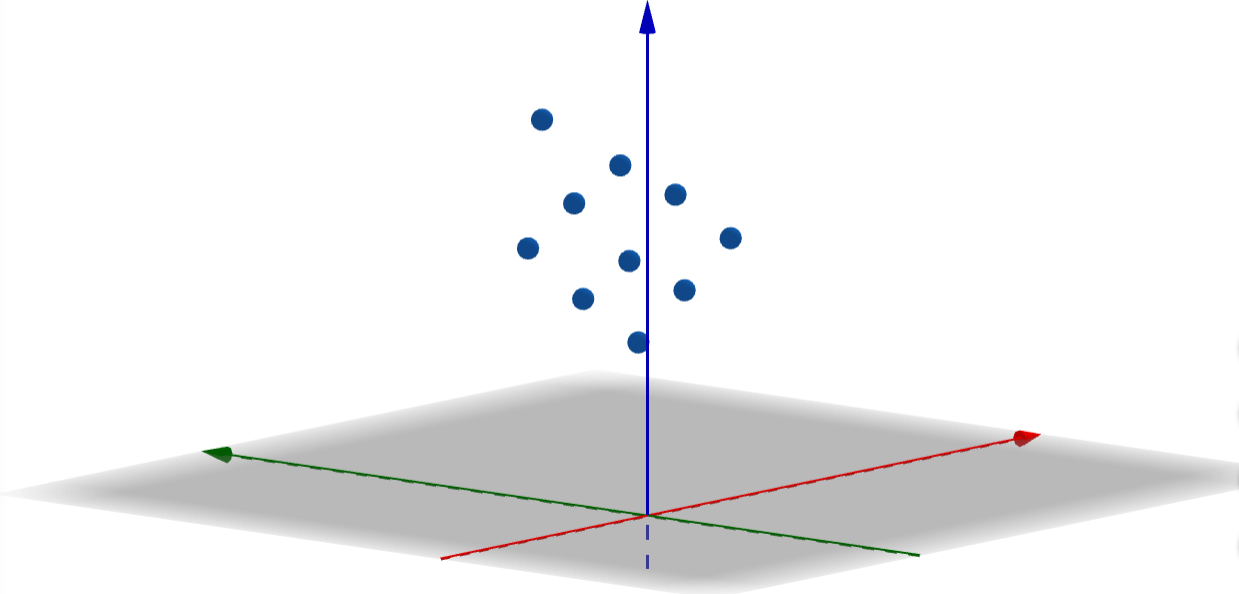
\includegraphics[width=5cm]{points.png}
    \end{minipage}
  \end{figure}


\end{frame}
    
\begin{frame}{Teorema Unificador}

  \vspace{0.3cm}

  Buscamos um problema de otimização que saibamos resolver e cuja solução também resolva outros problemas de otimização.

  \vspace{0.3cm} \pause

  \begin{figure}
    \centering
    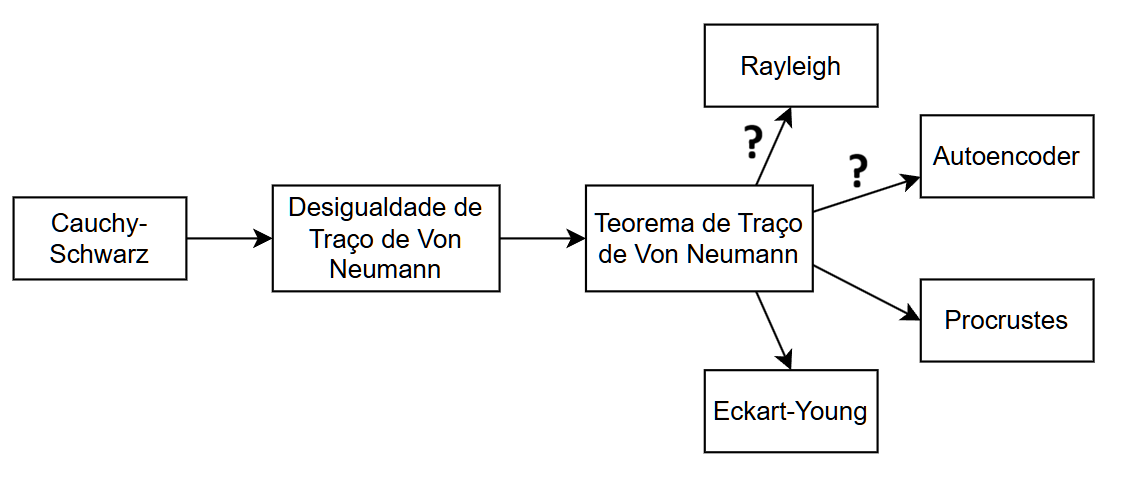
\includegraphics[width=11cm]{beautiful-tree.png}
  \end{figure}
\end{frame}


  \appendix
  % >8-------------------------------------REFERÊNCIAS-------------------------------------8<
\begin{frame}
  \frametitle{Referências}
  \nocite{*}
  \printbibliography
\end{frame}
% >8-------------------------------------REFERÊNCIAS-------------------------------------8<

% >8------------------------------------AGRADECIMENTOS-----------------------------------8<
\begin{frame}[plain]
  \centering
  \vspace{1cm}
  {\LARGE Raciocínio Equacional para a Derivação de \\ Algoritmos de Álgebra Linear sob a \\ Perspectiva de Otimização \par}
  \vspace{1cm}
  {\large João Victor Lopez Pereira \par}
  \vspace{0.5cm}
  {\large Daniel Sadoc Menasche \par}
  \vspace{0.5cm}
  {\large João Antonio Recio Paixão \par}
  \vfill
  {\footnotesize Pesquisa com bolsa CNPq-UFRJ \quad | \quad Tempo dedicado: 10 meses \par}
  \vfill
\end{frame}
% >8------------------------------------AGRADECIMENTOS-----------------------------------8<


\end{document}
